\section{Проектирование системы распределённых вычислений}

В данном разделе рассматриваются основные проектные решения,
определяющие построение разрабатываемой системы распределённых
вычислений. Сначала обосновывается выбор алгоритма консенсуса Raft,
затем описывается архитектура системы, включающая общую схему
взаимодействия компонентов, архитектуру Raft-узлов, клиентской части и
вычислительных узлов. Далее приводится обоснование выбора языка
программирования и инструментов реализации. Полная UML-диаграмма
классов для всех типов узлов приведена в Приложении~А.

\subsection{Обоснование выбора алгоритма консенсуса Raft}

Выбор алгоритма консенсуса является одним из ключевых проектных решений при
разработке отказоустойчивой системы распределённых вычислений. От выбранного
протокола зависят способ координации узлов, механизм репликации состояния,
поведение системы при отказах, а также сложность практической реализации и
сопровождения.

В исследовательской части были рассмотрены основные свойства алгоритмов Paxos и
Raft. Оба подхода обеспечивают согласованность данных и устойчивость к
частичным отказам, однако для проектируемой системы распределённых вычислений
существенное значение имеют не только теоретические гарантии, но и
архитектурные свойства алгоритма. Разрабатываемая система предполагает наличие
реплицируемого журнала операций, в котором должны фиксироваться события,
связанные с постановкой задач, изменением их состояния и подтверждением
выполнения. Следовательно, наиболее предпочтительным является алгоритм, в
котором журнал является центральной частью протокола, а его ведение и
согласование встроены в сам механизм консенсуса.

С этой точки зрения Raft лучше соответствует структуре разрабатываемой системы,
чем классический Paxos. В Paxos базовой единицей согласования является
отдельное значение, а построение полноценного реплицируемого журнала требует
дополнительных расширений и отдельного согласования механизма лидерства,
фиксации записей и восстановления после сбоев. В Raft, напротив, реплицируемый
журнал и выделенный лидер являются основой алгоритма. Это позволяет
естественным образом связать работу алгоритма консенсуса с управлением
состоянием кластера.

Важным аргументом в пользу Raft является также то, что для системы
распределённых вычислений наличие единственного лидера упрощает координацию.
Через лидера удобно выполнять регистрацию новых задач, упорядочение клиентских
запросов, фиксацию результатов и синхронизацию состояния между управляющими
узлами. При этом правила выборов, репликации и фиксации записей в Raft заданы
явно и не требуют введения дополнительных соглашений, выходящих за рамки
основного протокола.

С инженерной точки зрения Raft является более удобным и для практической
реализации. Его логика выражается через небольшое число ясно разделённых
механизмов: выбор лидера, поддержание лидерства, репликацию журнала и
продвижение индекса фиксации. Такое разделение упрощает проектирование
компонентов системы, обработку сбоев и сопровождение кода. Кроме того, широкое
распространение Raft в реальных системах подтверждает его практическую
пригодность для построения отказоустойчивых кластеров.

Итого, выбор алгоритма Raft обусловлен тем, что он наиболее полно соответствует
архитектуре проектируемой системы распределённых вычислений. Он обеспечивает
согласованность состояния узлов, поддерживает естественную модель
реплицируемого журнала, упрощает координацию кластера через выделенного лидера
и позволяет реализовать отказоустойчивую систему без введения избыточно сложных
вспомогательных механизмов.

\subsection{Архитектура системы распределённых вычислений}

\subsubsection{Общая архитектура системы}

На верхнем уровне архитектуры выделяются два класса узлов: узлы
консенсуса (Raft-узлы) и вычислительные узлы. Такое разделение
соответствует распространённой практике отделения контура управления, в котором
выполняются координация, согласование состояния и диспетчеризация, от
вычислительного контура, в котором осуществляется непосредственное выполнение
пользовательских задач \cite{coulouris2012}.

Raft-узлы образуют кластер, поддерживающий реплицированную машину
состояний. Они принимают клиентские запросы, выполняют их валидацию,
фиксируют изменения глобального состояния, принимают решения о постановке
задач в очередь и назначении задач вычислительным узлам. Вычислительные
узлы, в свою очередь, не участвуют в согласовании глобального состояния и
выполняют только назначенные им задачи, периодически сообщая о ходе
выполнения и возвращая результаты.

Общая архитектура приложения приведена на
рис.~\ref{fig:arch-overview}.

\begin{figure}
  \centering
  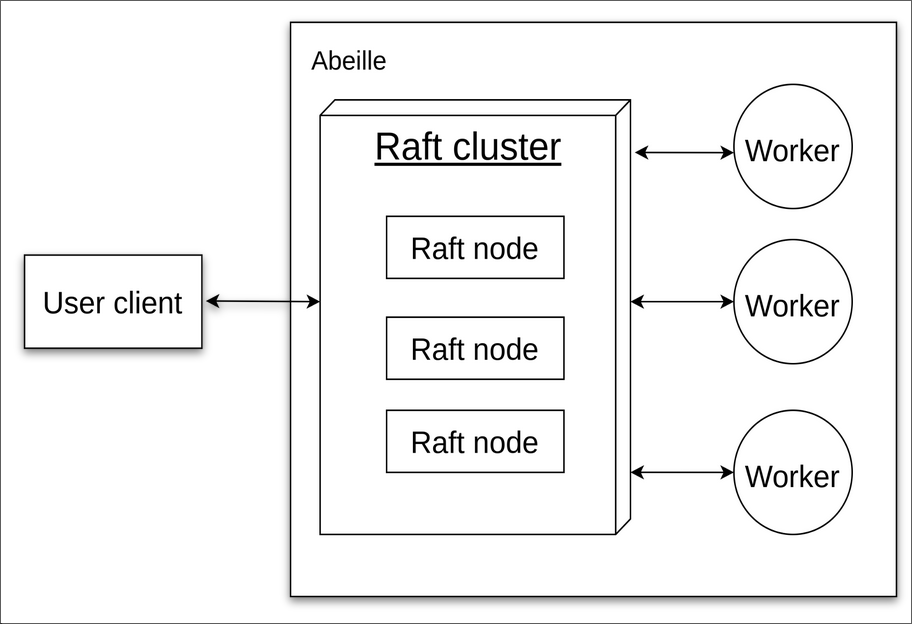
\includegraphics[scale=0.4]{inc/arch-overview.png}
  \caption{Высокоуровневая архитектура приложения}
  \label{fig:arch-overview}
\end{figure}

Клиент взаимодействует только с кластером Raft; запрос может быть принят любым
узлом и при необходимости переадресован лидеру. Каждая операция, влияющая на
состояние системы, сначала записывается в журнал кластера, подтверждается
кворумом узлов и только после этого применяется к реплицированной машине
состояний. Изменения состояния затем передаются в модуль диспетчеризации,
который назначает задачи конкретным вычислительным узлам. Аналогично,
результаты выполнения также проходят через кластер Raft до того, как становятся
доступными клиенту.

Такая схема позволяет обеспечить детерминированный порядок событий,
устойчивость к повторным сообщениям за счёт идемпотентных идентификаторов
задач и возможность повторного назначения задач при сбоях
вычислительных узлов без нарушения согласованности.

В архитектуре намеренно исключаются прямые связи между клиентом и
вычислительными узлами, а также горизонтальные связи между самими
вычислительными узлами. Это уменьшает связанность компонентов, снижает
радиус отказа и позволяет сосредоточить все изменения глобального
состояния в одном месте --- в кластере Raft. В результате упрощаются
контроль доступа, аудит, масштабирование и сопровождение системы, а
вычислительный контур остаётся относительно простым и легко расширяемым.

Система проектируется для модели аварийного завершения и восстановления
после сбоя в условиях частичной синхронности сети. Кластер Raft
обеспечивает безопасность, то есть отсутствие противоречивых
зафиксированных решений, при любой динамике обмена сообщениями и
живучесть при выполнении временных предположений \cite{ongario14}. При
отказе отдельного вычислительного узла незавершённые задания остаются
зафиксированными в состоянии и могут быть переназначены. При отказе
лидера выполняется переизбрание, после чего система продолжает
обслуживание запросов при наличии кворума. Такая конфигурация позволяет
сохранять работоспособность при недоступности до
$\lfloor (N-1)/2 \rfloor$ узлов кластера консенсуса, где $N$ --- число
Raft-узлов, что соответствует стандартной кворумной гарантии
\cite{lynch1996}.

При проектировании также рассматривались альтернативные варианты:
прямое взаимодействие клиента с вычислительными узлами,
полносвязная одноранговая сеть вычислительных узлов с децентрализованным
согласованием, а также объединение ролей, при котором каждый
вычислительный узел одновременно является участником консенсуса.
Указанные варианты были признаны менее подходящими, поскольку увеличивают
сложность обеспечения глобальной согласованности, усложняют
эксплуатацию и ухудшают масштабируемость. Предложенная архитектура
позволяет сохранить контур консенсуса компактным и управляемым, а
вычислительный контур --- эластичным и удобным для масштабирования.

\subsubsection{Архитектура Raft узлов}

Каждый узел кластера Raft содержит несколько функциональных модулей,
взаимодействие которых обеспечивает корректную обработку запросов и
поддержание согласованного состояния всей системы. Архитектура узла
изображена на рис.~\ref{fig:raft-overview}.

\begin{figure}
  \centering
  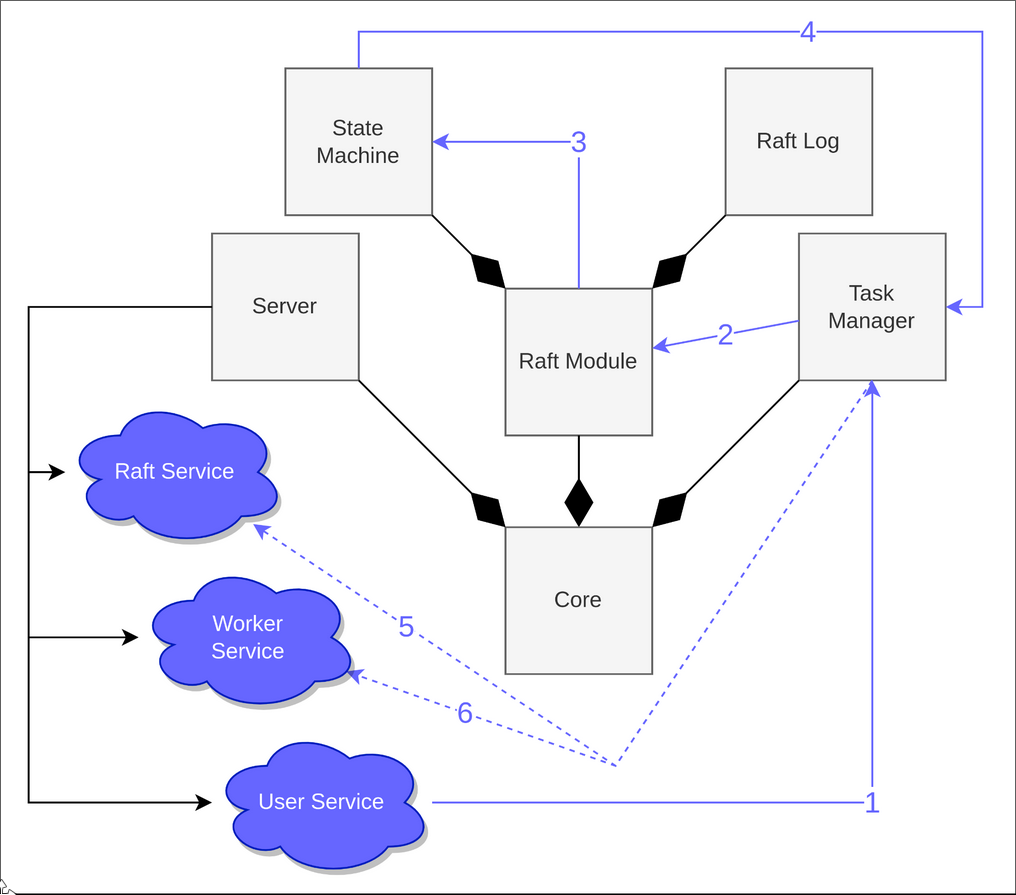
\includegraphics[scale=0.25]{inc/raft-arch.png}
  \caption{Архитектура Raft узла}
  \label{fig:raft-overview}
\end{figure}

Поток обработки клиентского запроса начинается с поступления данных в
\texttt{серверный модуль} узла-лидера. Сервер принимает запросы от
клиентов и маршрутизирует их во внутренние сервисы. В частности,
запросы, связанные с постановкой новых заданий на выполнение,
направляются в \texttt{пользовательский сервис (User Service)}. Этот
сервис выполняет первичную валидацию и подготовку данных, после чего
передаёт их в \texttt{менеджер заданий (Task Manager)}. Задача
менеджера заключается в выборе подходящего вычислительного узла,
исходя из состояния системы, доступности ресурсов и стратегии
планирования.

Поскольку система должна сохранять корректность работы даже при сбоях
отдельных узлов, менеджер заданий не отправляет задание
вычислительному узлу напрямую. Вместо этого сформированная операция
передаётся в \texttt{модуль Raft}, который отвечает за репликацию и
согласование состояния между всеми узлами кластера. Модуль Raft
добавляет операцию в \texttt{журнал Raft (Raft Log)}, где хранятся
ещё не зафиксированные изменения состояния. Далее эти записи
реплицируются на остальные узлы кластера посредством сообщений
лидера.

Когда большинство узлов подтверждает успешную запись данных в свои
локальные журналы, лидер считает запись зафиксированной, после чего
она применяется к \texttt{машине состояний (State Machine)}. Машина
состояний представляет собой детерминированный автомат, который
преобразует последовательность зафиксированных операций в текущее
состояние системы. За счёт применения одной и той же
последовательности команд на каждом узле достигается согласованность:
все реплики приходят к одинаковому состоянию независимо от того, какой
узел является лидером.

После того как запись зафиксирована и применена к состоянию, менеджер
заданий получает сигнал о возможности безопасного выполнения задания.
На этом этапе задание отправляется выбранному вычислительному узлу.
Результат выполнения также проходит через Raft: по завершении работы
вычислительный узел формирует ответ, который реплицируется и
фиксируется аналогично исходному запросу. Лишь после этого результат
считается подтверждённым и возвращается клиенту, что гарантирует
согласованность даже при сбоях в момент ответа.

Ключевым элементом узла является \texttt{ядро (Core)}, выполняющее роль
интеграционного слоя между модулями. Оно отвечает за инициализацию и
завершение работы компонентов, координирует обмен сообщениями между
ними и предоставляет единый интерфейс для внешнего управления узлом.

Такая архитектура обеспечивает согласованное и детерминированное
поведение системы при сбоях и гарантирует, что любая операция либо
будет зафиксирована на большинстве узлов, либо не повлияет на
глобальное состояние системы. Система остаётся работоспособной до тех
пор, пока доступно более половины узлов кластера, что соответствует
базовому требованию алгоритмов кворумного консенсуса.

\subsubsection{Архитектура клиентской части}

Клиентская часть системы обеспечивает пользователю интерфейс для
постановки задач на выполнение и получения результатов. Основными
компонентами клиентской стороны являются:
\begin{itemize}
    \item \texttt{конфигурационные данные задачи} --- входные параметры,
    описывающие вычислительную задачу, хранятся в формате JSON
    (например, \texttt{data.json});
    \item \texttt{библиотека задачи} --- бинарный модуль
    (\texttt{libtask.so}), содержащий реализацию функции обработки
    данных;
    \item \texttt{клиентское приложение (CLI)} --- консольная утилита,
    служащая интерфейсом между пользователем и распределённой
    системой.
\end{itemize}

Такой подход позволяет передавать в систему не только входные данные,
но и сам алгоритм обработки. В рамках прототипа предполагается
выполнение в среде Linux, поэтому пользовательская задача
представляется в виде динамической библиотеки формата
\texttt{.so}.

Процесс взаимодействия клиента с системой проходит следующие этапы
(см.~рис.~\ref{fig:client-arch}):
\begin{enumerate}
    \item Пользователь передаёт клиенту \texttt{data.json} и
    динамическую библиотеку \texttt{libtask.so}, после чего CLI
    формирует запрос, содержащий данные задачи и код её исполнения, и
    отправляет его в кластер Raft.
    \item Лидер кластера принимает запрос, реплицирует его и передаёт
    в подсистему диспетчеризации, которая назначает задачу конкретному
    вычислительному узлу. В запросе указывается уникальный
    идентификатор задачи для обеспечения идемпотентности.
    \item Клиент вычислительного узла получает задание и передаёт его
    на выполнение в среду исполнения, где подгружается
    \texttt{libtask.so} и запускается соответствующая функция с
    параметрами из \texttt{data.json}. После завершения выполнения
    результат формируется в сериализованном виде и отправляется
    обратно в кластер Raft для фиксации в состоянии.
    \item После фиксации результата в реплицированной машине состояний
    лидер Raft уведомляет клиента о завершении работы. CLI принимает
    ответ, сохраняет результат локально либо выводит пользователю в
    удобной форме.
\end{enumerate}

\begin{figure}
  \centering
  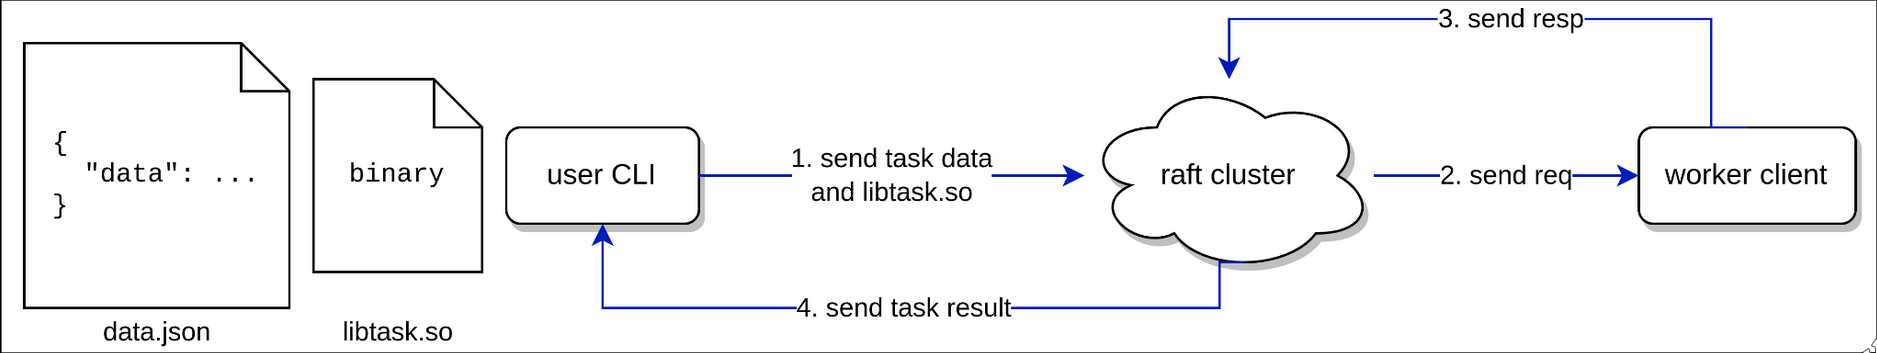
\includegraphics[scale=0.25]{inc/client-arch.png}
  \caption{Взаимодействие клиента с кластером}
  \label{fig:client-arch}
\end{figure}

Данная архитектура клиентской части обладает рядом преимуществ. Во-первых, она
универсальна, поскольку клиент не привязан к конкретному типу задач, и любое
вычисление, представленное в виде бинарной библиотеки с единым интерфейсом,
может быть передано в систему. Во-вторых, клиент имеет минимальные зависимости,
так как реализован в виде лёгкой утилиты, не требующей сложной конфигурации,
что упрощает её развёртывание и интеграцию в CI/CD. В-третьих, архитектура
обеспечивает надёжность, поскольку через механизм Raft проходят все изменения
глобального состояния задачи: постановка, назначение, фиксация результата и
регистрация ошибок.

Таким образом, клиентская часть системы выступает удобным и
унифицированным интерфейсом, который инкапсулирует сложность
взаимодействия с распределённой инфраструктурой и позволяет
пользователю сосредоточиться на определении вычислительных задач и
анализе результатов.

\subsubsection{Архитектура вычислительного узла}

Вычислительный узел предназначен для непосредственного выполнения
задач, поступающих из кластера Raft, и возврата результатов их
обработки. Архитектура такого узла организована так, чтобы обеспечить
изоляцию вычислений, устойчивость к сбоям и минимальное влияние
выполняемой задачи на стабильность основной службы.

Ключевыми компонентами вычислительного узла являются:
\begin{itemize}
    \item \texttt{главный процесс (main)} --- точка входа, отвечающая
    за инициализацию среды, запуск клиента вычислительного узла и
    менеджера процессов;
    \item \texttt{клиент вычислительного узла (worker client)} ---
    процесс, поддерживающий постоянное соединение с кластером Raft,
    принимающий задания на выполнение и уведомляющий менеджер о
    необходимости запуска исполняющего процесса;
    \item \texttt{менеджер (manager)} --- отдельный процесс,
    отвечающий за создание изолированных дочерних процессов, которым
    передаётся выполнение конкретных задач;
    \item \texttt{исполняющий процесс (mayfly)} --- лёгкий дочерний
    процесс, который загружает указанную динамическую библиотеку,
    выполняет функцию обработки данных и формирует результат.
\end{itemize}

Поток выполнения задачи организован следующим образом
(см.~рис.~\ref{fig:worker-arch}):

\begin{enumerate}
    \item Приём запроса. Клиент вычислительного узла получает
    задание из кластера Raft и подтверждает его приём.
    \item Создание рабочего процесса. Клиент вычислительного
    узла отправляет запрос менеджеру на создание нового исполняющего
    процесса. Менеджер выполняет \texttt{fork()}, создавая изолированный
    процесс.
    \item Загрузка библиотеки. Исполняющий процесс
    подгружает указанную пользователем библиотеку задачи.
    \item Выполнение задачи. Обработка входных данных
    производится внутри исполняющего процесса. В случае ошибки или
    аварийного завершения процесс завершается без влияния на основной
    клиент вычислительного узла.
    \item Отправка результата. После завершения выполнения
    результат возвращается менеджеру, который передаёт его обратно в
    клиент вычислительного узла.
    \item Репликация результата. Клиент вычислительного узла
    формирует ответ и отправляет его в кластер Raft для фиксации в
    реплицированной машине состояний.
\end{enumerate}

\begin{figure}
  \centering
  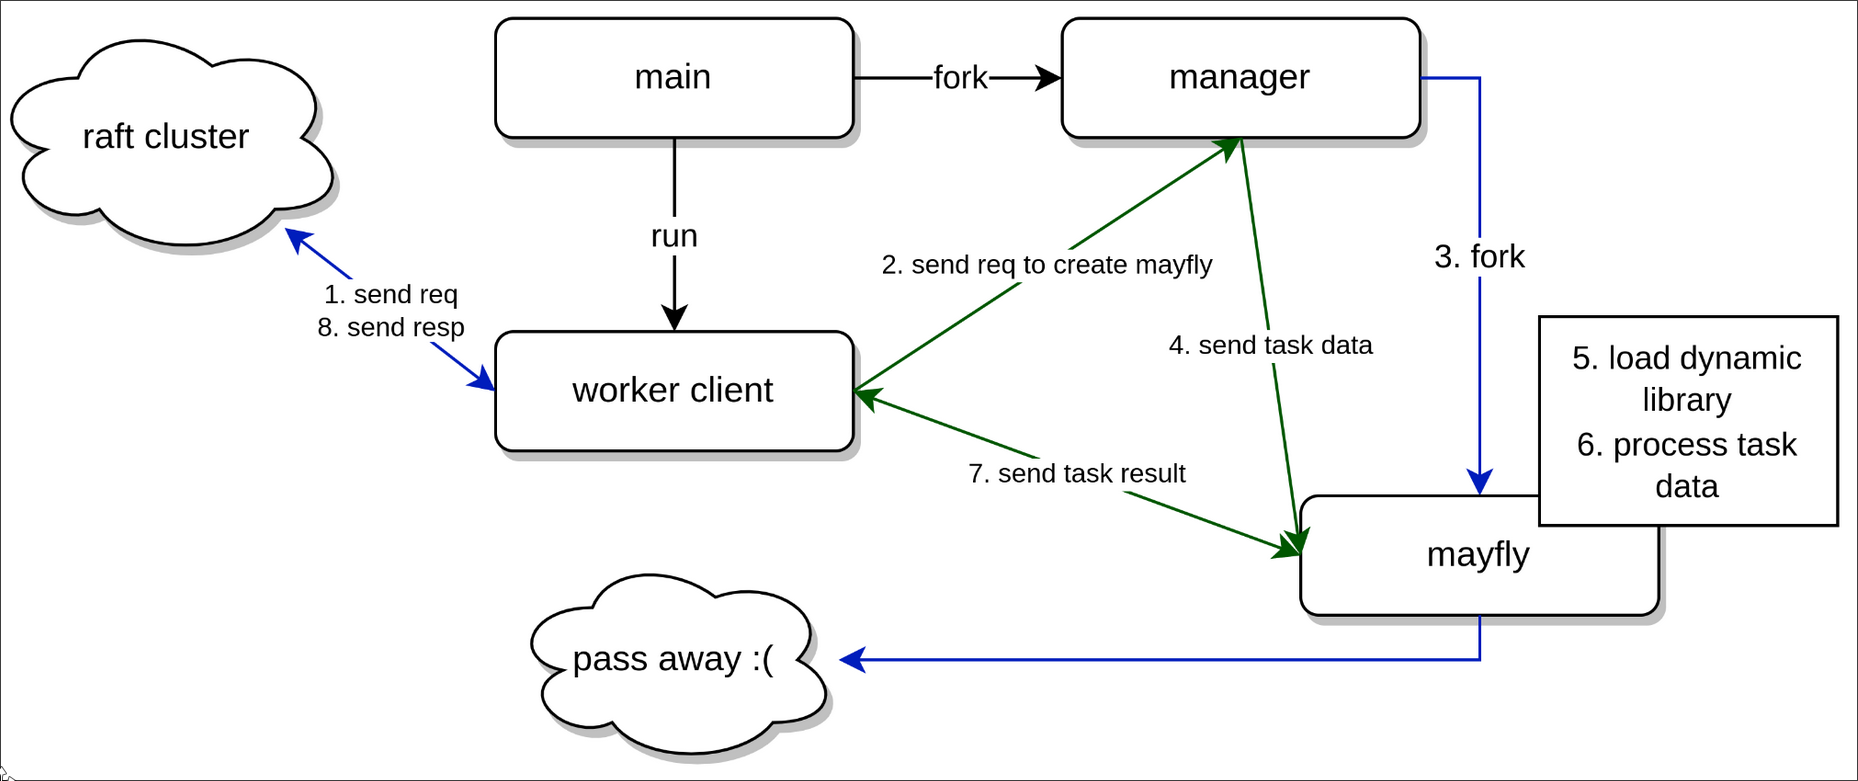
\includegraphics[scale=0.25]{inc/worker-arch.png}
  \caption{Взаимодействие вычислительного узла с кластером}
  \label{fig:worker-arch}
\end{figure}

Архитектура поддерживает модель <<одно задание --- один процесс>>. Это
обеспечивает изоляцию исполнения, поскольку сбой в задаче не влияет на
остальные процессы вычислительного узла. Кроме того, достигается
отказоустойчивость: при завершении дочернего процесса менеджер может корректно
обработать сбой, зарегистрировать ошибку и при необходимости запросить
повторное выполнение через кластер. Наконец, упрощается очистка ресурсов, так
как после завершения работы исполняющий процесс уничтожается вместе с
выделенными ему ресурсами, что исключает накопление неосвобождённых ресурсов.

Такое построение вычислительного узла обеспечивает гибкость и
устойчивость всей системы, позволяя безопасно выполнять пользовательский
код, динамически масштабировать количество обрабатываемых задач и
гарантировать возврат результата даже при частичных сбоях.

\subsection{Выбор языка программирования и инструментов реализации}

Для реализации системы распределённых вычислений был выбран язык
программирования C++, а в качестве основных инструментов
взаимодействия между компонентами --- стек gRPC и Protocol
Buffers. Такой выбор обусловлен требованиями к
производительности, управлению ресурсами, строгой типизации
интерфейсов и удобству построения распределённого взаимодействия
между узлами кластера. Использование контейнеров стандартной
библиотеки C++, в частности \texttt{std::deque} при реализации
Raft-лога, также соответствует данному выбору языка и позволяет
гибко управлять внутренними структурами данных.

Выбор C++ обусловлен несколькими причинами. Во-первых, данный язык
предоставляет высокую производительность и предсказуемый контроль над памятью,
что важно для серверных компонентов, постоянно обрабатывающих сетевые
сообщения, управляющих очередями задач и поддерживающих состояние
реплицируемого журнала. Во-вторых, C++ позволяет строить многопоточные
приложения с использованием стандартных средств синхронизации и контейнеров,
что особенно важно при реализации конкурентных компонентов распределённой
системы. В-третьих, язык обладает развитой экосистемой библиотек для сетевого
взаимодействия и хорошо интегрируется с промышленными средствами описания
интерфейсов и сериализации данных.

Для организации сетевого взаимодействия между узлами был выбран стек
\texttt{gRPC + Protocol Buffers}.Он обеспечивает эффективную и строго
типизированную коммуникацию между распределёнными компонентами системы.

gRPC представляет собой высокопроизводительную платформу удалённого вызова
процедур. Использование HTTP/2 позволяет поддерживать постоянные соединения,
двунаправленные потоки и мультиплексирование запросов, что удобно для
взаимодействия между компонентами распределённой системы. Для рассматриваемой
архитектуры это особенно важно, поскольку управляющие узлы, клиентская часть и
вычислительные узлы должны регулярно обмениваться сообщениями различного типа:
от служебных уведомлений и команд консенсуса до запросов на постановку и
выполнение вычислительных задач.

Protocol Buffers используется как средство описания интерфейсов и сериализации
данных. В системе \texttt{.proto}-файлы выступают единым формальным описанием
сообщений и контрактов взаимодействия как между клиентом и кластером, так и
между внутренними компонентами. Это уменьшает вероятность ошибок согласования
интерфейсов, упрощает сопровождение системы и позволяет автоматически получать
строго типизированные структуры данных и код сетевого взаимодействия. Кроме
того, Proto-схемы также используются для описания записей Raft-лога, что делает
выбранный формат единым для внутренних и внешних обменов.

Выбранный технологический стек даёт следующие практические преимущества для
разрабатываемой системы:
\begin{itemize}
    \item единое описание сообщений и интерфейсов для всех взаимодействующих
компонентов;
    \item строгую типизацию и автоматическую генерацию значительной части
сетевого кода;
    \item высокую производительность обмена данными и поддержку параллельных
соединений;
    \item удобство развития протокола взаимодействия без полной переработки
существующей реализации.
\end{itemize}

Таким образом, выбор C++ в сочетании с gRPC и Protocol Buffers обусловлен
требованиями проектируемой системы распределённых вычислений к
производительности, надёжности и удобству сопровождения. Данный набор
технологий позволяет реализовать как внутреннее взаимодействие узлов
консенсусного кластера, так и внешние интерфейсы работы с вычислительными
задачами в рамках единой и строго типизированной архитектуры.
